\graphicspath{{results/fig/}}

\chapter{Results}

\section{Data logging}
The resulting GPS coordinates that were stored to the micro-SD card during the data logging test were plotted on a map of Stellenbosch, and are shown in red in Fig.\ref{fig:rooi-plane-loop}.
The actual path that was travelled was a loop starting on the corner of Victoria and Ryneveld street, then a left turn onto Bosman street, a left turn onto Merriman avenue and 
a left turn back onto Ryneveld street. 

\begin{figure}[!h]
    \centering
    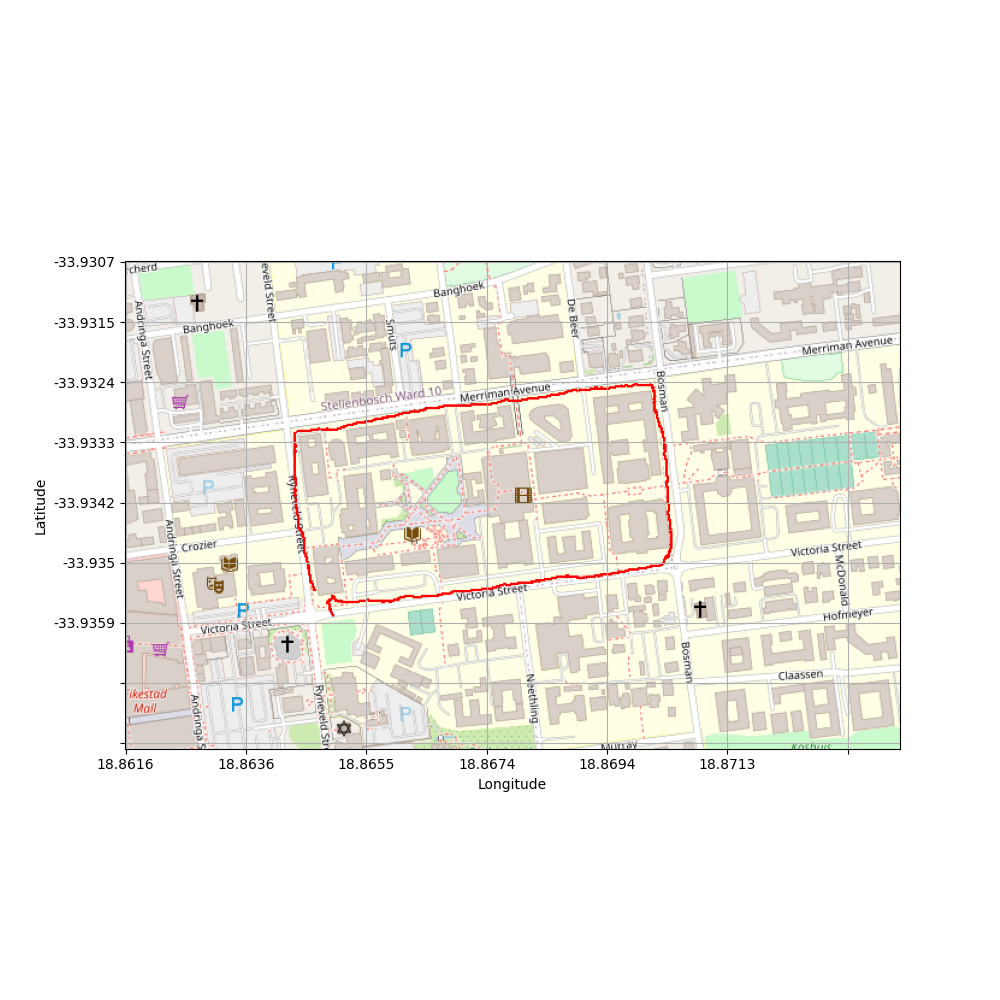
\includegraphics[width=0.8\linewidth]{rooi_plane_loop.png}
    \caption[Data logging test]{GPS coordinates of path travelled}
    \label{fig:rooi-plane-loop}
\end{figure}

The GPS coordinates correspond approximately to the actual path that was travelled, and the accuracy of the GPS receiver is therefore sufficient for the purposes of this project. These results 
have also verified the data logging capabilities of the system. 

\section{Digital Compass}
Two separate tests where done to test the accuracy of the digital compass. The results of the first test are shown in Fig.\ref{fig:digital-compass-test-1}. The error between the digital compass
and the handheld compass is shown in Fig.\ref{fig:digital-compass-test-1-error}. The average error was calculated to be $6.7312^{\circ}$. The error can be attributed to a inadequate calibration
process - compass rotation does not cover all possible angles, calibration process too short or sample frequency used not high enough.

\begin{figure}[!h]
    \centering
    \begin{subfigure}[!h]{=0.9\linewidth}
        \centering
        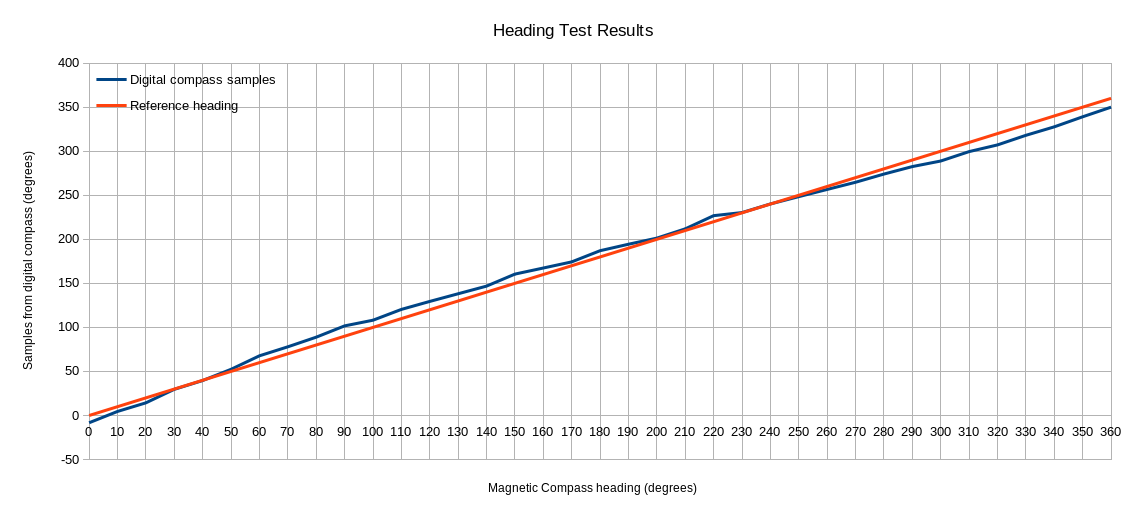
\includegraphics[width=1\linewidth]{digital-compass-test-1.png}
        \caption{Digital compass heading compared to handheld compass heading}
        \label{subfig:digital-compass-test-1}
    \end{subfigure}

    \begin{subfigure}[!h]{=0.9\linewidth}
        \centering
        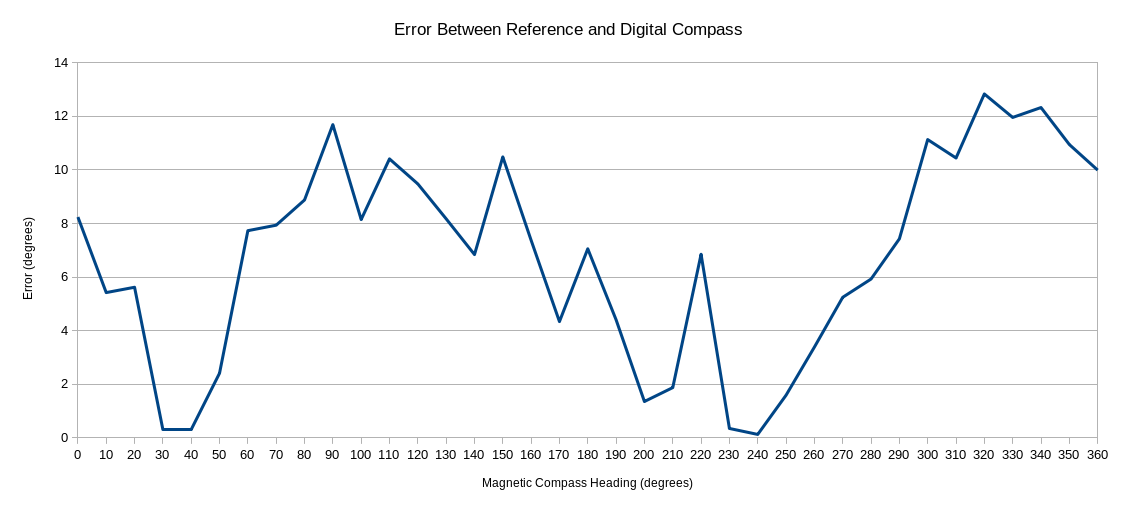
\includegraphics[width=1\linewidth]{digital-compass-test-1-error.png}
        \caption{Error between Digital compass heading and handheld compass heading}
        \label{subfig:digital-compass-test-1-error}
    \end{subfigure}
    \caption[Digital compass accuracy test-1]{Digital compass accuracy test}
    \label{fig:Digital compass accuracy test-1}
\end{figure}

The test was therefore redone, this time an extensive calibration of the digital compass was done. The results of the second test are shown in Fig.\ref{subfig:digital-compass-test-2}. The error 
between the digital compass and the handheld compass is shown if Fig.\ref{subfig:digital-compass-test-2-error}. The average error for this test was calculated as $1.5091^{\circ}$. The results of
this test verify that the digital compass is accurate when placed on a flat surface.

\begin{figure}[!h]
    \centering
    \begin{subfigure}[!h]{=0.9\linewidth}
        \centering
        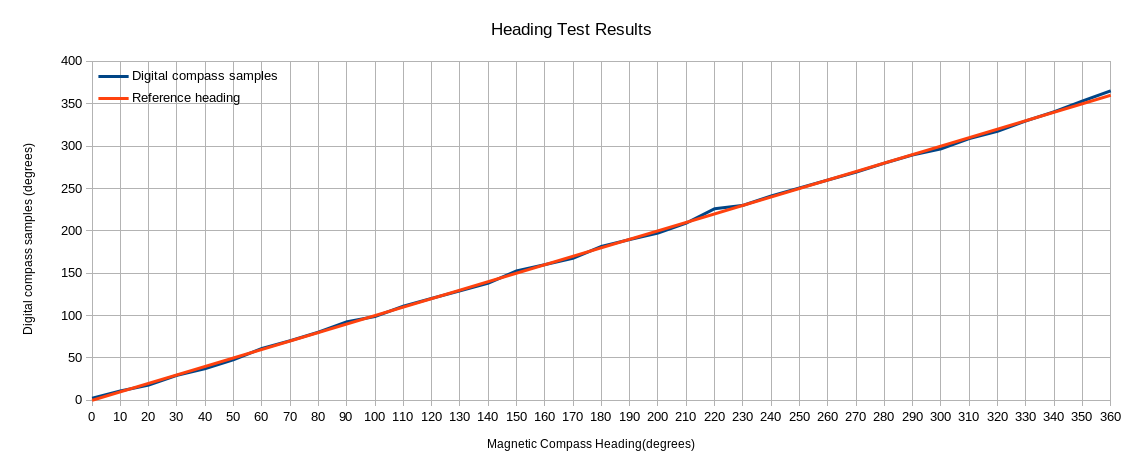
\includegraphics[width=1\linewidth]{digital-compass-test-2.png}
        \caption{Digital compass heading compared to handheld compass heading}
        \label{subfig:digital-compass-test-2}
    \end{subfigure}

    \begin{subfigure}[!h]{=0.9\linewidth}
        \centering
        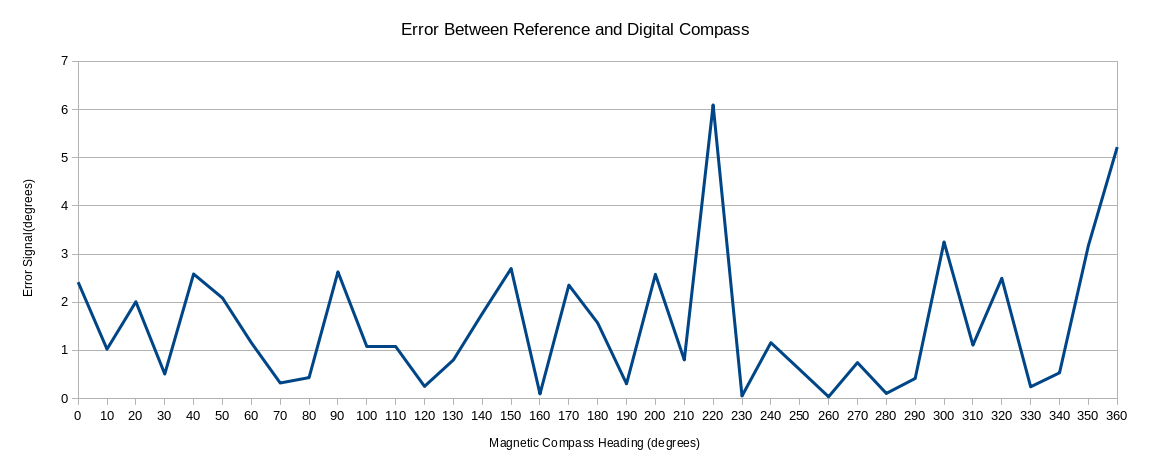
\includegraphics[width=1\linewidth]{digital-compass-test-2-error.png}
        \caption{Error between Digital compass heading and handheld compass heading}
        \label{subfig:digital-compass-test-2-error}
    \end{subfigure}
    \caption[Digital compass accuracy test-2]{Digital compass accuracy test}
    \label{fig:Digital compass accuracy test-2}
\end{figure}

The results of the tilt compensation test are shown in Fig.\ref{subfig:tilt-comp-error}. It should be noted that this test was conducted using the same calibration values (hard-iron offset and 
soft-iron correction values) that were determined and used in Fig.\ref{fig:Digital compass accuracy test-1}. The results of the tilt compensation test are therefore compared to the results of 
the test done in Fig.\ref{fig:Digital compass accuracy test-1}. 

\begin{figure}[!h]
    \centering
    \begin{subfigure}[!h]{=0.9\linewidth}
        \centering
        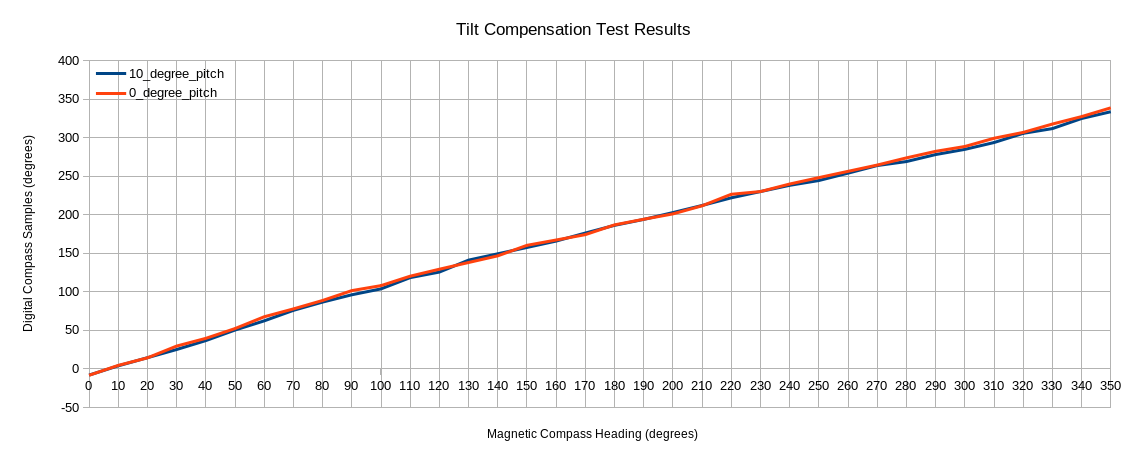
\includegraphics[width=1\linewidth]{tilt-comp-test.png}
        \caption{Tilt compensated digital compass heading compared to handheld compass heading}
        \label{subfig:tilt-comp-test}
    \end{subfigure}

    \begin{subfigure}[!h]{=0.9\linewidth}
        \centering
        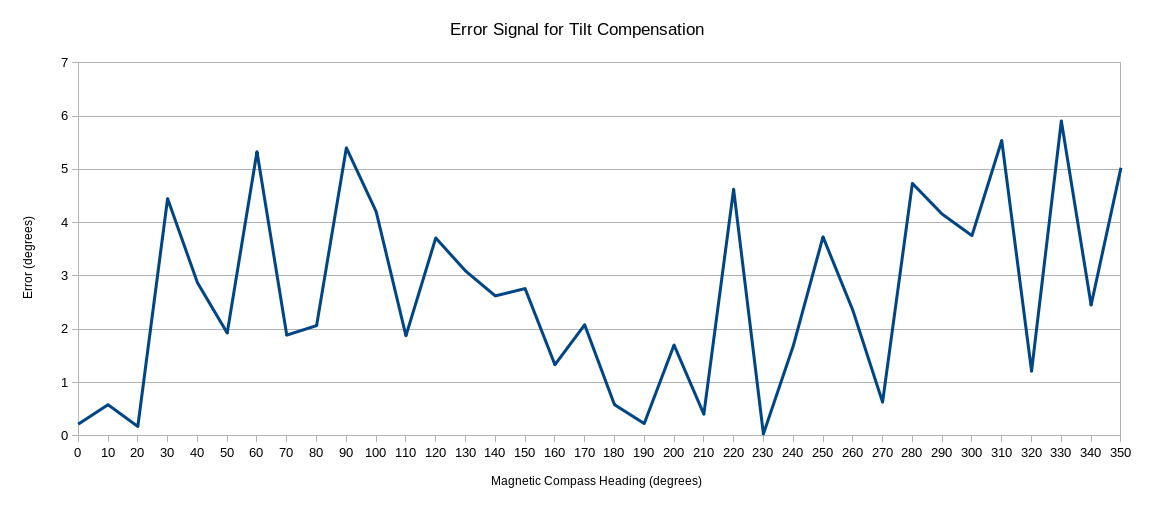
\includegraphics[width=1\linewidth]{tilt-comp-test-error.png}
        \caption{Error between tilt compensated digital compass heading and handheld compass heading}
        \label{subfig:tilt-comp-error}
    \end{subfigure}
    \caption[Tilt compensation test]{Tilt compensation algorithm test}
    \label{fig:tilt-comp}
\end{figure}

The tilt-compensated digital compass readings are approximately equal to the results obtained when the digital compass had a pitch angle of zero. The error in the results seen in Fig.\ref{subfig:tilt-comp-error}
can be attributed to the slight difference in angle when adjusting the wooden platform by hand between the $10^{\circ}$ steps. The average error was found to be equal to $2.6502^{\circ}$. The calculations done
in section \ref{sec: ...} show that the samples taken at varying degrees of pitch angle should theoretically be the same. The results shown in Fig.\ref{fig:tilt-comp} show that the tilt compensation 
algorithm does work.

\section{Rudder control}

The results of the rudder control test which was conducted out of the water are shown in Fig.\ref{fig:rudder-control-dry}. The average value of reference heading is $44.603^{\circ}$ and the average value of actual 
heading is $44.728^{\circ}$. These values are approximately equal and therefore the error signal that is generated for the rudder controller should keep the vessel on course when on the water. The variance of the 
actual heading during the test was calculated as $13.178^{\circ}$, which can be attributed to slight sway when walking.  

\begin{figure}
    \centering
    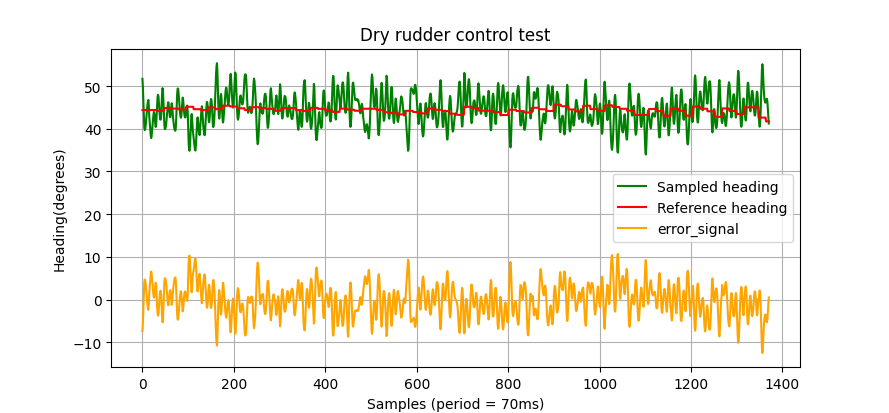
\includegraphics[width=1\linewidth]{dry-rudder-test.png}
    \caption[Rudder control test out of water]{Results of rudder control test out of water}
    \label{fig:rudder-control-dry}
\end{figure}

For the first rudder control test conducted on the water, the apparent wind was determined before hand to be roughly $100^{\circ}$, the sail position was therefore set to $40^{\circ}$.%NB must work this out using updates sail position formulae i.e. one with new pwm_min value 
The target coordinate given to the system corresponded to a location on the side of the dam. The proportional gain factor was set to 1.5 and integral gain factor was set to zero. The GPS 
coordinates logged during the test were plotted with Python and are shown in Fig.\ref{fig:rudder-control-test-1-path}. 


\begin{figure}
    \centering
    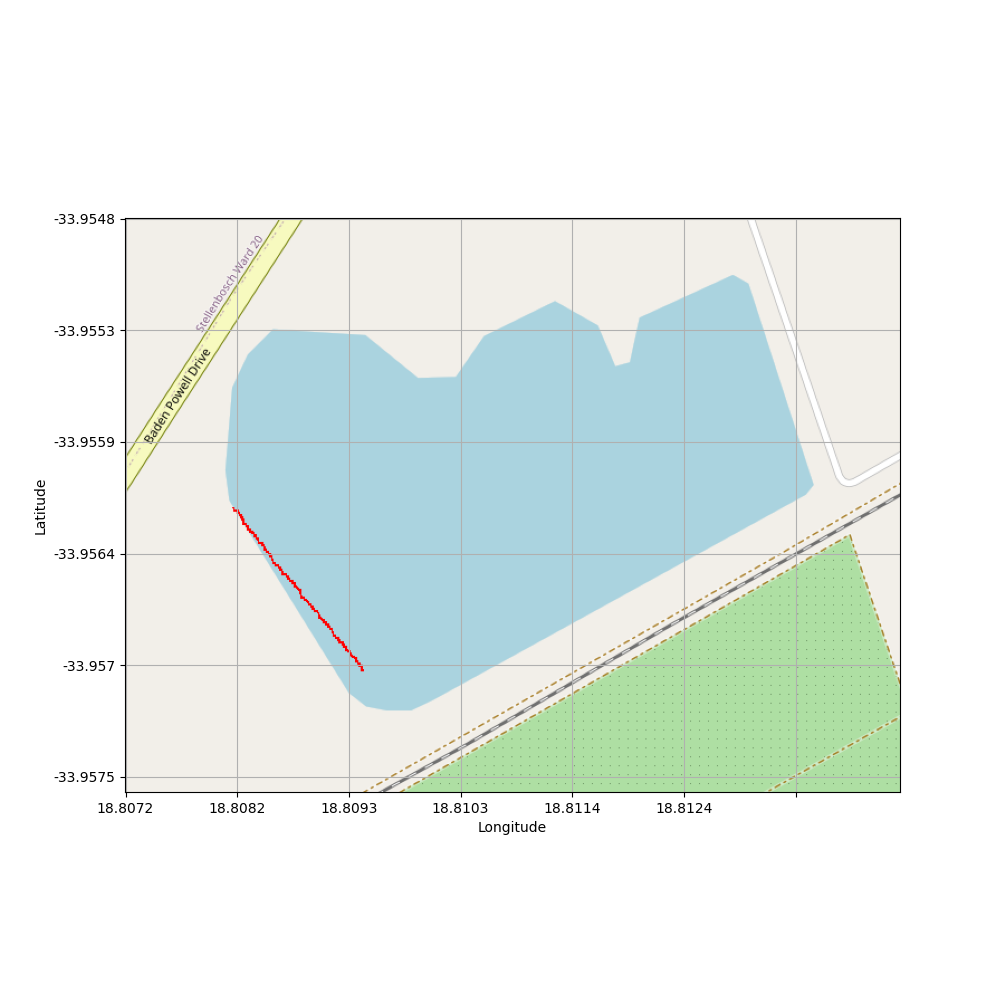
\includegraphics[width=0.8\linewidth]{dam-test-1/dam-test-1.png}
    \caption[Path travelled in first rudder control test]{GPS coordinates of path travelled}
    \label{fig:rudder-control-test-1-path}
\end{figure}

 
During the test the vessel was visibly oscillating from starboard to port side, this can be seen when analyzing Fig.\ref{subfig:first-rudder-control-heading}, which is a plot of the measured 
heading and reference heading data, logged throughout the test. The average reference heading value is $111.866^{\circ}$, and the average sampled heading value is $115,404^{\circ}$. The variance 
of the sampled bearing is $216,495^{\circ}$. The oscillation indicates that the proportional gain factor is too high and overshoot is occurring. 

\begin{figure}
    \centering
    \begin{subfigure}{=0.9\linewidth}
        \centering
        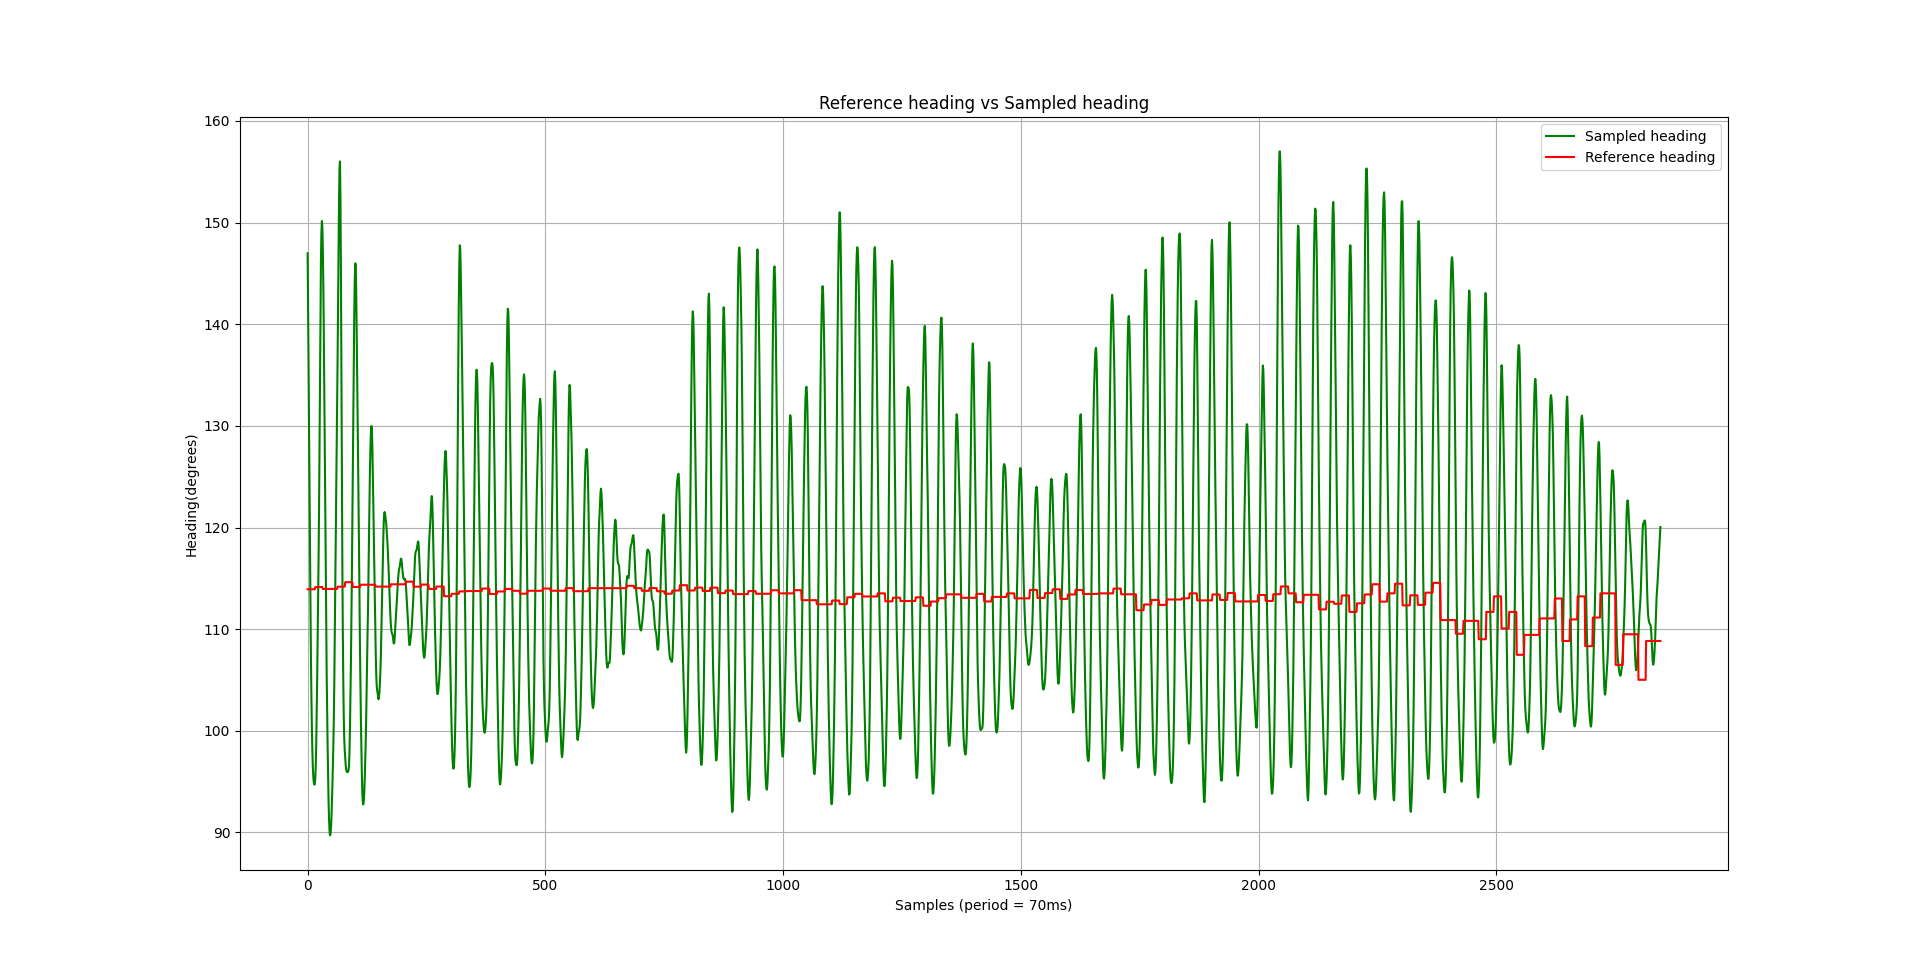
\includegraphics[width=1\linewidth]{dam-test-1/heading.png}
        \caption{sampled and reference heading}
        \label{subfig:first-rudder-control-heading}
    \end{subfigure}

    \begin{subfigure}{=0.9\linewidth}
        \centering
        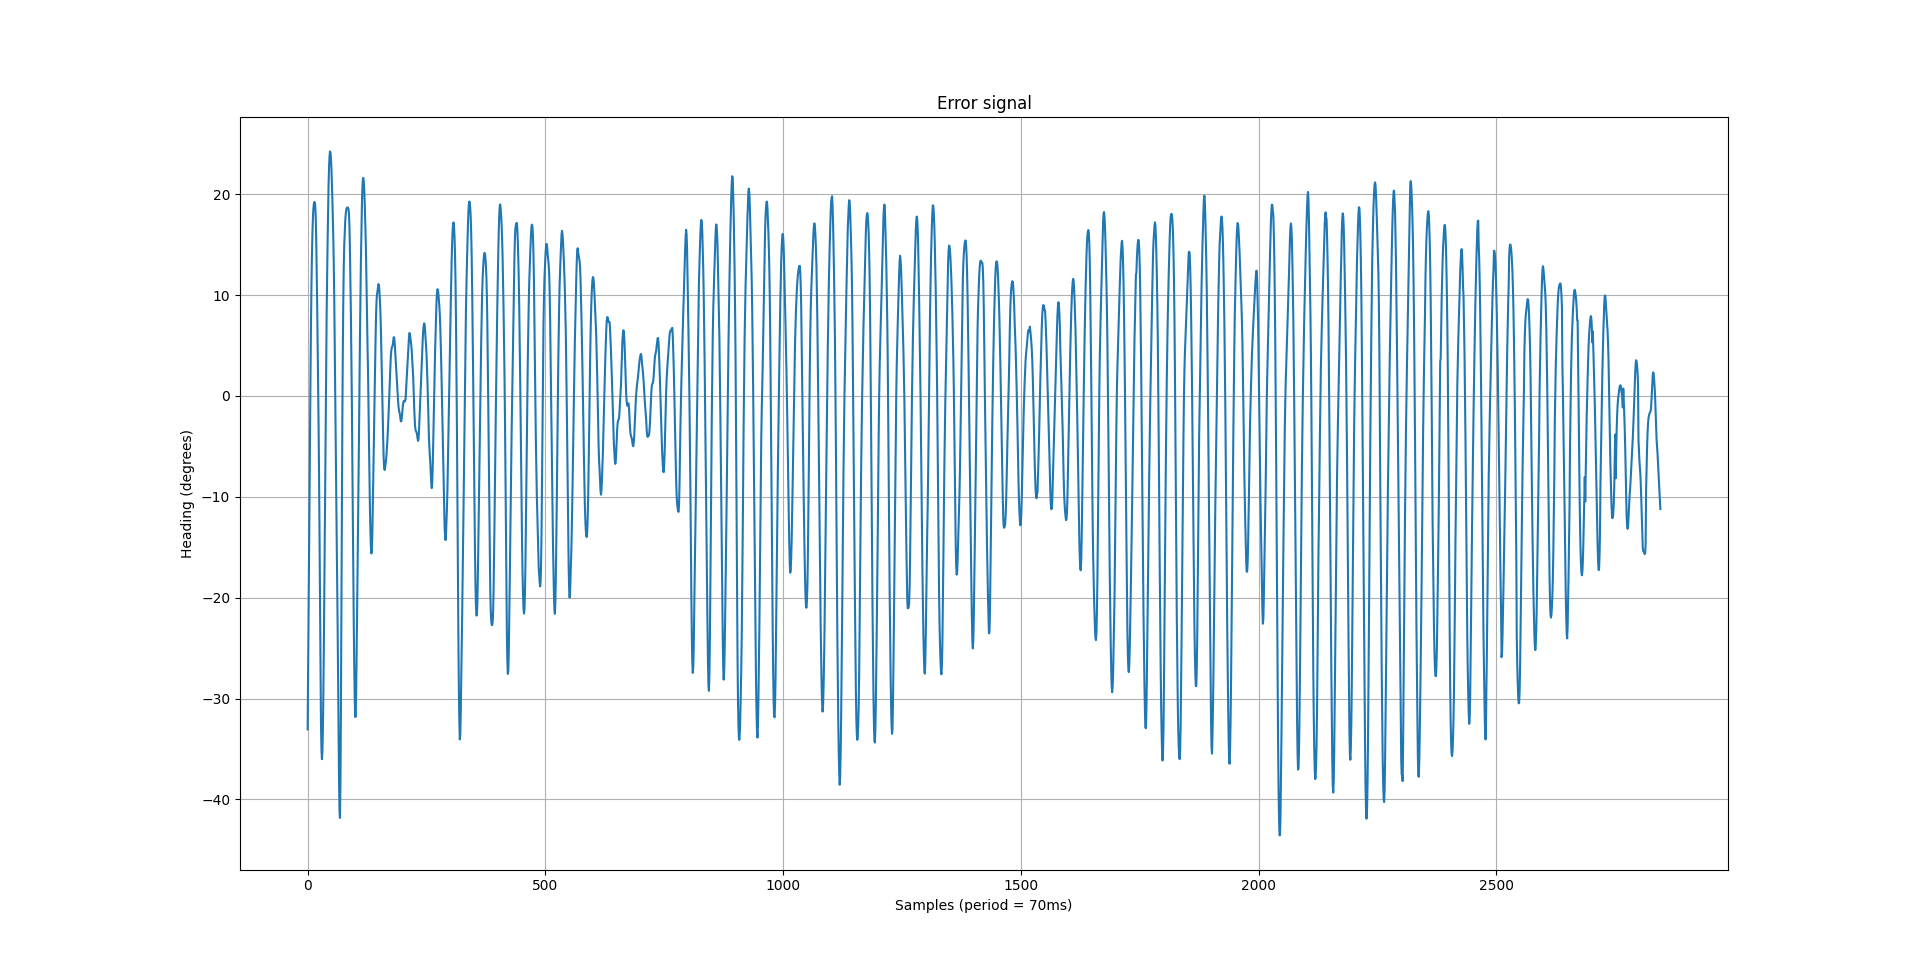
\includegraphics[width=1\linewidth]{dam-test-1/error-signal.png}
        \caption{Error signal}
        \label{subfig:first-rudder-control-error}
    \end{subfigure}

    \begin{subfigure}{=0.9\linewidth}
        \centering
        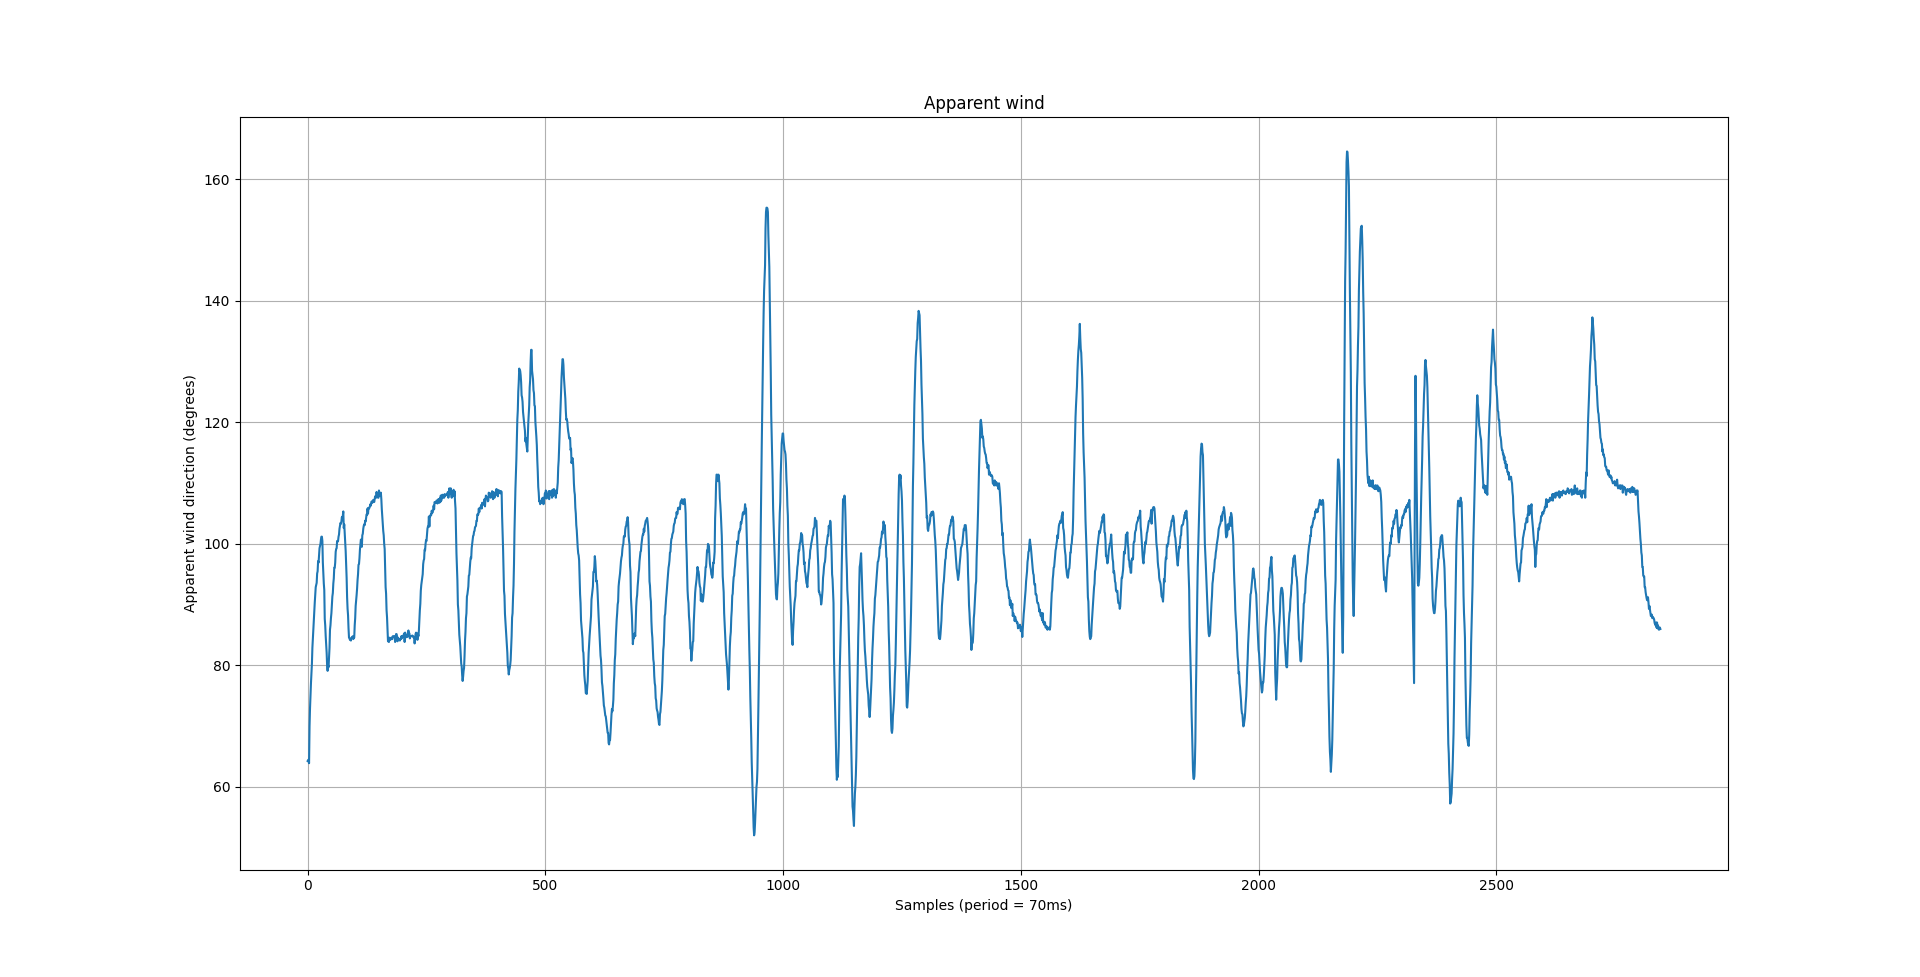
\includegraphics[width=1\linewidth]{dam-test-1/apparent-wind.png}
        \caption{Apparent wind}
        \label{subfig:first-rudder-control-error}
    \end{subfigure}

    \caption[First rudder control test on water]{First rudder control test on water}
    \label{fig:first-rudder-control-water}
\end{figure}


The error signal, which is input to the rudder 
controller is shown in Fig.\ref{subfig:first-rudder-control-error}. The maximum speed reached during the test was 1.161 knots. Although the sail controller was not implemented during this test, 
wind direction readings were still taken and the data is illustrated in Fig.\ref{subfig:first-rudder-test-wind}. The average apparent wind value is $98.8^{\circ}$, which corresponds to the initial 
wind direction reading that was taken. The variation in apparent wind direction throughout the test can be attributed to the oscillating of the vessel.